\kapitola{Analýza problému}
Tato kapitola se zabývá analýzou funkčních a nefunkčních požadavků pro softwarové řešení. Požadavky vznikaly na základě konzultace s vedoucím a vlastní invencí.

\sekce{Funkční požadavky}
Funkční požadavky jsou rozděleny do několika kategorii.

\podsekce{Simulace}
Vyhodnocování agenta bude probíhat jeho nasazením v simulovaném prostředí. Fitness bude pak vyhodnocena na základě jeho akcí v prostředí.
\begin{itemize}
	\item Testovací prostředí musí být pro všechny agenty stejné
	\item Fitness funkce musí být deterministická
	\item Fitness by měla být zjistitelná kdykoliv v průběhu simulace
	\item Simulace by měla být konfigurovatelná 
	\item Možnost změny obtížnosti simulace pro agenta
	\item Měla by existovat možnost spuštění více instancí simulace v rámci jednoho programu
\end{itemize}
\podsekce{Vizualizace}
Průběh algoritmu je třeba zobrazit.
\begin{itemize}
	\item Je třeba provést grafickou vizualizaci fyzikální simulace
	\item Při zobrazení by mělo být možné vyčíst stav agenta (fitness, senzory, ...) 
	\item Možnost vizualizace průběhu simulace v reálném čase (například pro její demonstraci v předmětu VUI2)
\end{itemize}

\podsekce{Experimenty}
Práce zahrnuje vyhodnocování agenta v různých podmínkách z tohoto vychází následující požadavky:

\begin{itemize}
\end{itemize}

\sekce{Nefunkční požadavky} 
Spolu s funkčními požadavky jsou na řešení kladeny také požadavky nefunkční.
\begin{itemize}
	% TODO: Předělat do formátu Něco - ....
	\item Škálovatelnost - Možnost spustit a vykreslit libovolné množství simulací
	\item Rychlost simulace. - Simulace by měla být schopná samostatně běžet alespoň rychlostí 30 snímků za vteřinu.
	\item Robustnost - Simulace by měla být odolná neočekávaným situacím
	\item Portabilita - bylo třeba zajistit, aby šlo kód rozběhnout v různých platformách v různých konfigurací.
	\item Robustnost - Simulace by si měla poradit s neočekávanými vstupy, jako je třeba \textbf{NaN}, který vychází z neuronové sítě.
\end{itemize}

\kapitola{Návrh řešení}


\kapitola{Implementace}
Vlastní práce se skládá ze dvou částí klientská část, která slouží k~vizualizaci algoritmu a zobrazení výsledků ze serverové části. Serverová část pro maximální urychlení simulace. 

\kapitola{Simulace}
Simulace je realizovaná jako knihovna pro Node.js, lze jí tedy použít jak u klientské částí, tak u serverové části. Poskytuje kompletní fyzikální simulaci agenta, prostředí ve kterém se pohybuje, jeho ovládání a výpočet fitness funkce. Součástí simulačního prostředí je také kód pro její vizualizaci.

Při návrhu simulace bylo dbáno především na následující kriteria:

\begin{enumerate}
	\item Rychlost - Simulace musí být, co nejrychlejší s ohledem na to, že jich bude třeba pustit tisíc pro vyhodnocení jediné generace
	\item Nenáročnost - Simulace musí běžet na různém hw v různých konfiguracích (viz sekce \ref{sec:cluster})
	\item Robustnost - Simulace by si měla poradit s neočekávanými vstupy, jako je třeba \textbf{NaN}, který vychází z neuronové sítě
	\item Stejné prostředí - Simulace musí poskytovat stejné prostředí pro všechny jedince
	\item Portabilita - bylo třeba zajistit, aby šlo kód rozběhnout v různých platformách v různých konfiguracích.
	\item Škálovatelnost - Možnost spustit a vykreslit libovolné množství simulací
\end{enumerate}

Rychlost byla zajištěna implementací profilovacího programu (\textbf{benchmark.js} ve složce simulation), který spouští simulaci na předem připravené populaci jedinců. Výstupem je pak doba, za jakou jí vyhodnotil na jednom jádře procesoru. Tento údaj byl pak používán při implementaci simulace pro orientační představu, jak moc případné změny v kódu ovlivňují rychlost samotné simulace. Dále byla simulace podrobena občasnému profilování v klientské částí s pomocí vývojářských nástrojů prohlížeče chrome, na kterém simulace jede nejlépe.

Nenáročnost, která souvisí s rychlostí pak byla zajištěna tím, že bylo v průběhu psaní kódu dbáno na to, aby v průběhu simulace nedocházelo k přebytečným alokacím, které by nejen že mohli způsobit přebytečný nárůst požadované paměti ale způsobovali by také nepředvídatelné zpomalení, které s sebou přináší jazyk využívající garbage kolektor.

Robustnost je podrobněji vysvětlená v sekci \ref{sec:fitness} a popis toho, jak bylo dosaženo stejných podmínek pro všechny agenty lze nalézt v návrhu \ref{sec:ECS} především v popisu RoadManageru.

\sekce{Části ECS použité v simulaci}
\label{sec:ECS}
Simulace je implementovaná v duchu ECS (\textbf{Entity component system}) podrobný popis lze nalézt v sekci \ref{sec:ces}. Není tedy žádným překvapením, že se všechny komponenty nalezené v simulaci dají rozložit na systémy, komponenty a entity. Pro lepší představu o implementaci je níže uveden přehled všech systému, entit a komponent použitých v simulaci.

\podsekce{Entity}
Simulace obsahuje následující entity:

\textbf{PhysicsGroup} Seskupuje fyzikální entity do jedné pro snadnou manipulaci s nimi.

\textbf{RoadPart} Entita, která obaluje jednu nebo více překážek tak, aby se s nimi dalo snadno pohybovat používá se pro tvorbu složitějších dílů vozovky.

\textbf{Car} Reprezentuje samotné vozidlo obsahuje jak jeho grafickou reprezentaci, tak kompletní logiku a fyzikální model.
 
\podsekce{Komponenty}
Simulace obsahuje následující komponenty:
\textbf{Car} obsahuje všechny potřebné informace o agentovi. Toto zahrnuje vše od neurnové sítě, která je použitá pro jeho řízení po ovládání jednotlivých kol agenta.

\textbf{Graphics} komponenta, která obsahuje grafické informace pro \textbf{Pixi.js}.

\textbf{Physics} komponent, která obsahuje fyzikální entity pro \textbf{P2.js}

\podsekce{Systémy}
Simulace obsahuje následující systémy:

\textbf{Car} systém, který se stará o ovládání agenta a částečně o vyhodnocování jeho fitness.

\textbf{Graphics} grafický systém, který slouží především k překreslování entit s pomocí \textbf{PIXI.js}

\textbf{Physics} krokuje fyzikální engine a synchronizuje grafickou reprezentaci s fyzikální entitou. Tento proces probíhá pro každý snímek a skládá se z přiřazení nové rotace a pozice pro grafickou entitu.

\textbf{RoadDirector} Road director se stará o generování nekonečného prostředí pro agenta. Děje se tak na základě předefinovaných dílu vozovky z nichž každý zaplňuje celou obrazovku simulace. V případě, že agent dorazí až na konec obrazovky je mu určen nový navazující dílek. Agent je pak přehozen na opačnou stranu obrazovky a zároveň je vyměněn díl na kterém se nachází.
Hlavní výhodou tohoto přístupu je to, že agent může jezdit po vozovce donekonečna bez starosti o to, že by se dostal na limit fyzikálního enginu (přetečení pozice fyzikálního objektu). Další nesporná výhoda tohoto přístupu je úspora paměťových nároků, kterou by s sebou nesla definice větší mapy a možnost generování náhodných map pro testování agenta.

\sekce{Fitness funkce}
\label{sec:fitness}
Fitness funkce je důležitou součástí simulace, která zásadně ovlivňuje chování výsledných agentů a je tedy nutné jí volit vhodně. Je nutné, aby funkce agenta motivovala ke správné činnosti.

Po několika pokusech a konzultaci s vedoucím práce byla jako metrika úspěchu agenta zvolena celková vzdálenost, kterou je agent schopný překonat v průběhu jedné generace. Výpočet je realizován s pomocí RoadDirectoru, který si při každém přechodu zaznamená bod, ve kterém se po přesunu agent nachází. Výsledná fitness je pak součet uražených vzdáleností pro každou místnost. Road direktor si pro každou obrazovku uchovává vzdálenost, kterou agent v dané obrazovce překonal. Výsledným fitness je pak součet všech vzdáleností na všech obrazovkách

Agenta je ovšem kromě motivace třeba také penalizovat za akce, které jsou nepřípustné. V případě simulace se jedná především o kolizi s překážkou, za což je agent penalizován předčasným ukončením simulace a nemožností tedy zvýšit svoji fitness.

\podsekce{Agent}
Definice samotného agenta zásadně ovlivňuje výsledek simulace, protože stanovuje vstupy a výstupy do a z~neuronové sítě. 

Samotným agentem je auto, které je vybaveno 6 vzdálenostními senzory. Měření těchto senzorů je normalizováno (maximální vzdálenost měřícího paprsku je 800 m) a předáno jako vstup do neuronové sítě.

Agent se poté každý snímek s~pomocí neuronové sítě \ref{fig:control_network} rozhoduje, jakou akci podnikne. Má následující možnosti:

\begin{enumerate}
	\item Ovládání volantu 
	\begin{enumerate}
		\item $z_1$ Otočení volantem o určitý počet stupňů doleva
		\item $z_2$ Otočení volantem o určitý počet stupňů doprava
	\end{enumerate} 
	\item Rychlostní stupně
	\begin{enumerate}
		\item $z_3$ - zpátečka
		\item $z_4 - z_6$ - rychlosti dopředu
	\end{enumerate}
\end{enumerate}

Ovládání volantu i volba rychlostního stupňů probíhá zároveň a to tak, že se vždy z dané skupiny neuronů vybere ten, který má největší hodnotu. Tento přístup je identický tomu, který se používá například u neuronových sítí pro klasifikaci.

\begin{figure}[h!]
	\centering
	\begin{neuralnetwork}[height=7]
		\newcommand{\nodetextx}[2]{\ifthenelse{\equal{#2}{0}}{$b_0$}{$s_{#2}$}}
		\newcommand{\nodetextz}[2]{$z_#2$}
		\newcommand{\nodetexth}[2]{\ifthenelse{\equal{#2}{0}}{$b_1$}{$h_{#2}$}}
		\inputlayer[count=6, title={Data ze senzorů}, text=\nodetextx]
		\hiddenlayer[count=6, title={Skrytá vrstva}]
		\linklayers
		\outputlayer[count=6, title={Výstup}, text=\nodetextz] 
		\linklayers
	\end{neuralnetwork}
	\caption{Neuronová síť agenta}
	\label{fig:control_network}
\end{figure}

\kapitola{Serverová část}
Serverová část vyhodnocuje jednotlivé jedince distribuovaně s~pomocí fronty úkolů. Frontu poskytuje knihovna \textbf{bull}, která používá \textbf{redis} pro správu údajů o~jednotlivých úkolech.

Cílem byl návrh robustního systému, který v~ideálním případě rozloží výpočetní zátěž mezi jednotlivé uzly rovnoměrně. Dalším požadavkem byla možnost odpojení kdykoliv kteréhokoliv z počítačů, jelikož ne všechny bylo možné nechat běžet přes noc.

\sekce{Výpočetní cluster}
\label{sec:cluster}
Ukázalo se, že vyhodnocování simulace zabírá neúměrné množství času a to i na nejvýkonnějším dostupném počítači. 
Například vyhodnocení jedné generace populace o~1024 jedincích zabralo ~290 s~na nejsilnějším dostupném pc. Z~tohoto důvodu bylo rozhodnuto o~distribuce výpočetní zátěže mezi více počítačů. Byl vytvořen výpočetní cluster se specifikací popsanou v~tabulce \ref{table:hw_table}.
\begin{table}[h!]
	\centering
	\begin{tabular}{|l|c|c|c|}
		\hline 
		Procesor & RAM & Počet & Architektura\\ 
		\hline 
		S5P6818 Octa core & 1 GB & 2 & arm64 \\ 
		\hline 
		Broadcom BCM2837B0 quad-core & 1 GB & 1 & arm32 \\ 
		\hline 
		Phenom X4 965 & 8 GB & 1 & x64 \\ 
		\hline
		Intel Core i5-2300 & 4 GB & 1 & x64 \\ 
		\hline
		AMD A4-4300M & 4 GB & 1 & x64 \\ 
		\hline 
		Intel atom x5-Z8350 & 2 GB & 1 & x64 \\ 
		\hline
		Cortex-A5 & 1 GB & 1 & armv7l \\
		\hline
	\end{tabular} 
	\caption{Použitý hardware}
	\label{table:hw_table}
\end{table}

\podsekce{Docker swarm}
Pro snadnou distribuci a správu byly všechny počítače zorganizovány do docker swarmu. Docker swarm obsahoval jednoho managera (Broadcom BCM2837B0 quad-core), který zároveň spouštěl klientskou aplikaci a další služby:

\begin{enumerate}
	\item \textbf{Portainer} pro správu clusteru
	\item \textbf{Arena} webové ui pro správu \textbf{bull}
	\item \textbf{redis} používaný knihovnou \textbf{bull}
\end{enumerate}

Použití docker swarmu umožňuje především snadné nasazení a správu zpracovávajících procesů. Zároveň zajišťuje, že všechny instance zpracovatelů mají unifikovanou konfiguraci, což je zvláště důležité pro dosažení konzistentních výsledků.

\sekce{Průběh vyhodnocování}
Serverová část pracuje dle diagramu \ref{fig:distributed}, kde je vidět, že klient zadává do fronty úkoly (genom a nastavení simulace). Jednotliví zpracovatelé (počítače v~clusteru), kteří si je z~ní vyberou, jednotlivé genomy vyhodnotí a hodnotu fitness funkce pošlou zpět na klienta. 

Jakmile klient dostane všechny hodnoty zpět provede na populaci genetický algoritmu (mutace, křížení, \dots) a poté je nová generace poslána znovu na vyhodnocení.

\begin{figure}[h!]
	\centering
	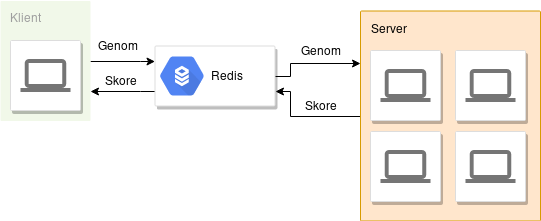
\includegraphics[scale=0.5]{distributed}
	\caption[Schéma distribuovaných výpočtů]{Schéma distribuovaných výpočtů}
	\label{fig:distributed}
\end{figure}

Tento přístup má několik výhod a to:

\begin{enumerate}
	\item Robustnost - Pokud jeden nebo více zpracovatelů selže (je například odpojen ze sítě) je možné pokračovat ve vyhodnocování (neúspěšný úkol lze vrátit zpátky do fronty). Toto v kombinaci s výše zmíněným docker swarmem znamená, že jakýkoliv výpočetní uzel lze kdykoliv vypnout a po znovu zapojení do sítě si načte nejnovější konfiguraci a začne znovu vyhodnocovat bez potřeby jakékoliv manipulace s jakoukoliv částí swarmu.
	\item Dobré rozložení zátěže - Jelikož si zpracovatel vytahuje úkoly z~fronty, je vždy optimálně zatížen, a není třeba řešit rozložení mezi různě výkonnými a zatíženými počítači.
	\item Škálovatelnost - problém lze škálovat až do doby, kdy počet procesorů nepřesáhne počet potřebných simulací. Chceme-li tedy vypočítat generaci o tisíci jedincích můžeme na ně nasadit až tisíc procesorů.
\end{enumerate}

Lze i namítnout, že se zde projevuje určitá režie při síťové komunikaci se serverem, což může být zdrojem určitého zpomalení. Nicméně se toto zpomalení neprojevilo v~průběhu testování clusteru. Právě naopak bylo naměřeno 10 násobné zrychlení oproti výpočtu na jednom počítači.

\kapitola{Klientská část}
Klientská část byla navržena tak, aby byla schopná vizualizovat průběh algoritmu NEAT a zároveň měla možnost znovu vyhodnocení existujících genomů vygenerovaných serverovou částí. První požadavek vznikl na základě konzultace s vedoucím, který chtěl algoritmus neurovoluce demonstrovat v hodinách předmětu VUI2. Druhý požadavek vznikl z důvodu potřeby vizualizace řešení, které generoval sever.

\sekce{Vizualizace}
Vizualizace se skládá z jednoduchého rozhraní, které lze vidět na obrázku \ref{fig:visualization}. V horní části je graf, zobrazující průběh genetického algoritmu. Lze v něm nalézt fitness nejlepšího, nejhoršího a průměrného jedince v populaci.

Další část se skládá z konfigurovatelného množství simulačních prostředí. Jednotliví jedinci v generaci jsou pak rovnoměrně rozloženi mezi všechna simulační prostředí a uživatel může pozorovat vývoj jedinců v realném čase.

Poslední tlačítko slouží k urychlení simulace. Způsobí to, že se simulace začne obnovovat bez vykreslování. Toto jí značně zrychlí.

\begin{figure}[h!]
	\centering
	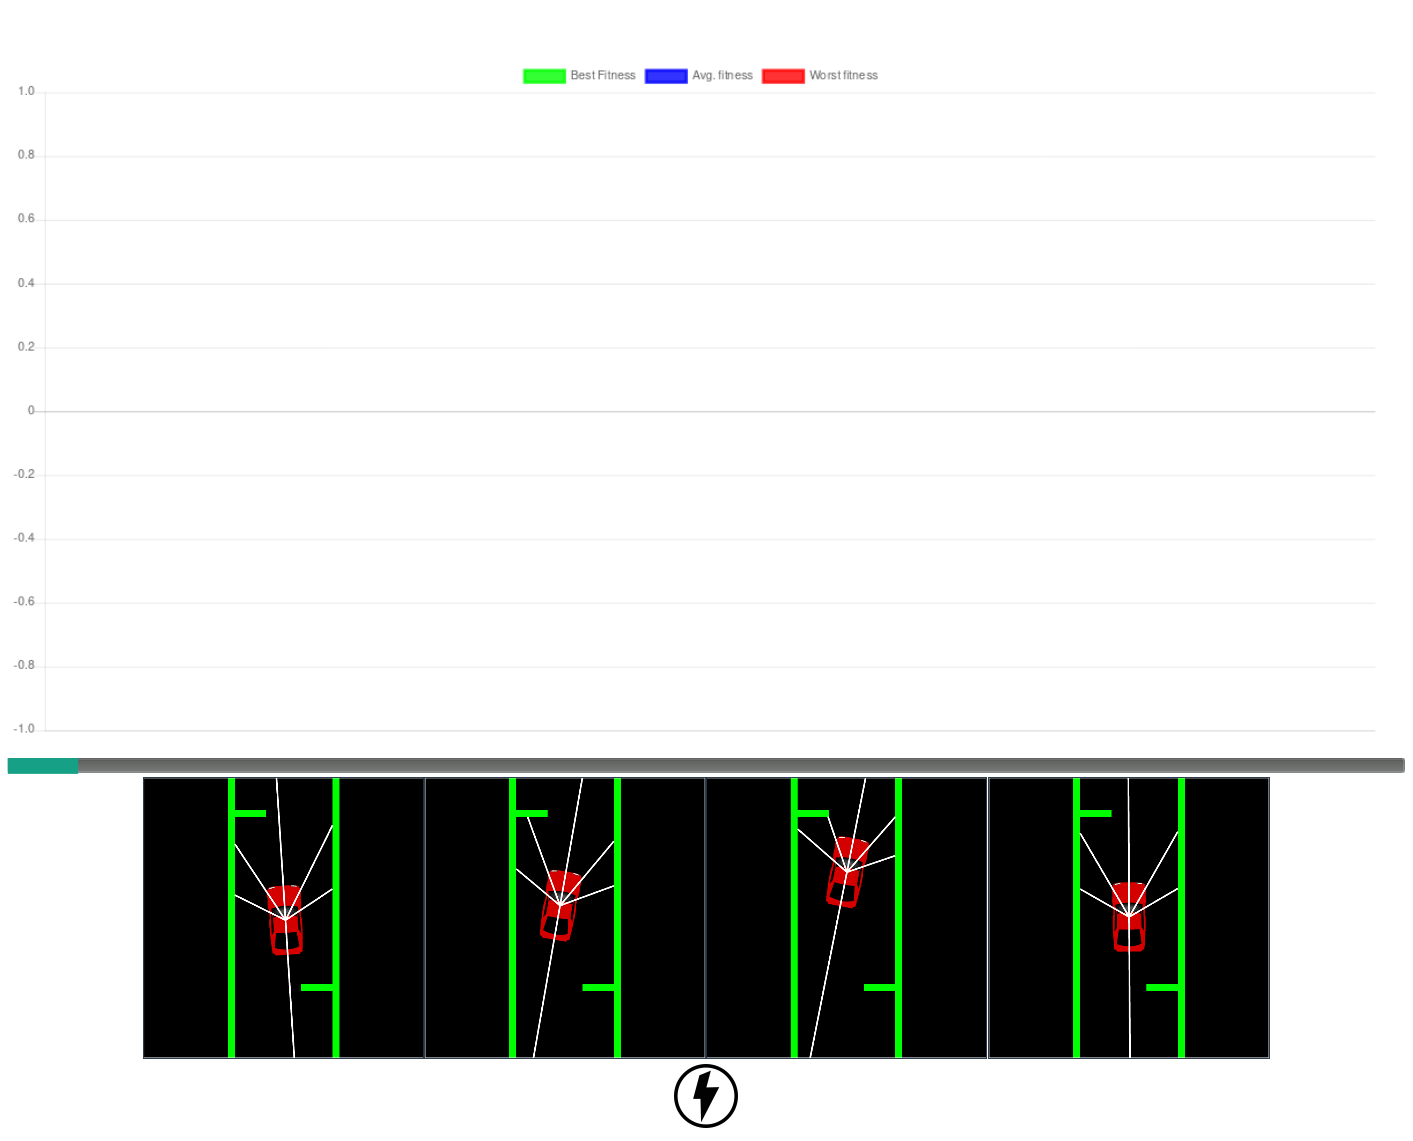
\includegraphics[width=0.6\linewidth]{visualization}
	\caption{Uživatelské rozhraní klientské části}
	\label{fig:visualization}
\end{figure}


\kapitola{Experimenty}
Po návrhu simulačního prostředí byl agent vyzkoušen v~několika situacích se stupňující se obtížností. Každá simulace probíhala s~1000 jedinci po 2000 generací. Ačkoliv je pravděpodobné, že by delší doba evaluace by pravděpodobně vyústila v lepší výsledky její výpočet v různých konfiguracích se ukázal jako příliš časově náročný navíc empirické pozorování ukázalo, že tato konfigurace poskytuje dostatečně dobré výsledky za snesitelný čas. 

S ohledem na časovou náročnost výpočtů (výpočet tisíce generací trvá na výpočetním clusteru přibližně 5 hodin) byly zkoumany jen tyto konfigurace:
\sekce{Nekonečná silnice ve tvaru I}
Agent byl umístěn do nekonečné rovné silnice ve tvaru I. Cílem bylo pozorovat, zda se agent bude schopný naučit řídit rovně. Agent po tisící generací dosáhl fitness 3 500 a naučil úspěšně kývavým pohybem udržet uprostřed vozovky.
\begin{figure}[h]
	\centering
	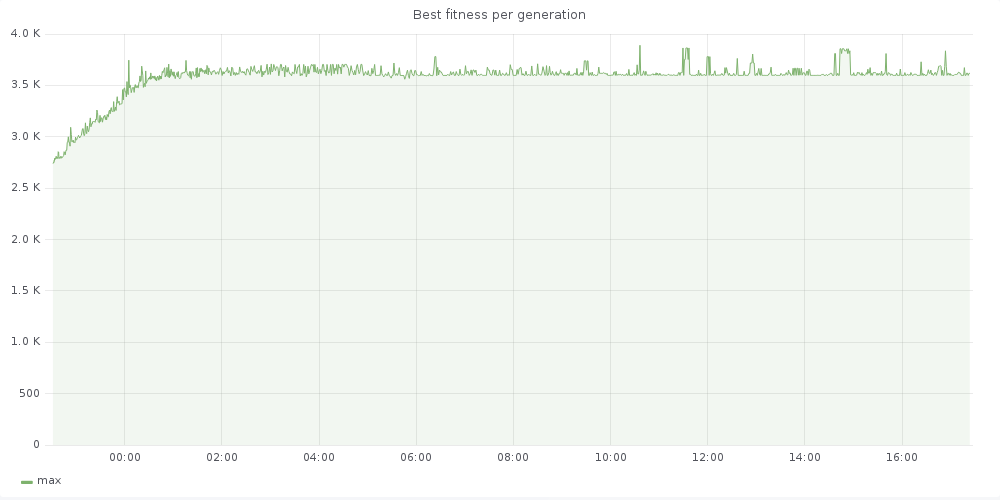
\includegraphics[scale=0.4]{I_fitness}
	\caption{Fitness agenta v průběhu času}
	\label{fig:i-experiment}
\end{figure}

\kapitola{Možná vylepšení}
Tato kapitola se bude zabývat možnými vylepšení současného řešení.
\kapitola{Závěr} 